%!TEX encoding = UTF-8 Unicode
\documentclass[master,korean,final]{cbnu-ecs}

% kaist.cls 에서는 기본으로 dhucs, ifpdf, graphicx 패키지가 로드됩니다.
% 추가로 필요한 패키지가 있다면 주석을 풀고 적어넣으십시오,
%\usepackage{...}
%

%\usepackage{kotex}
\usepackage{multirow}
\usepackage{varwidth}
\usepackage{amsmath}

%\renewcommand\tablename{표}
%\renewcommand\figurename{그림}

\newtheorem{theorem}{Theorem}	

% @command title 논문 제목
% @options [default: (none)]
% - korean: 한글제목 | english: 영문제목
\title[korean]{선분 카메라쌍 알고리즘을 이용한 사각형 특징의 기하학적 자세 추정을 통한 확장 칼만필터 기반 비주얼 SLAM}
\title[english]{Extended Kalman Filter based Visual SLAM with Geometric Pose Estimation of a Rectangle Feature using Coupled Line Camera Algorithm}

\author[korean] {이}{재 민}
\author[english]{Lee}{Jaemin}

\advisor[major]{박 찬 식}{Chan sik Park}{signed}

\department{RO}

% @command studentid 학번
\studentid{2014298010}

% 논문제출일9999kk,./
\submitdate{2016}{5}{1}

% @command approvaldate 지도교수논문승인일
% @param   year,month,day 연,월,일 순으로 입력
\approvaldate{2016}{6}{15}

% @command refereedate 심사위원논문심사일
% @param   year,month,day 연,월,일 순으로 입력
\refereedate{2016}{6}{1}

% @command gradyear 졸업년도
\gradyear{2016}{8}

% 본문 시작
\begin{document}


% 목차 (Table of Contents) 생성
\tableofcontents

% 영문초록 (abstract)
\begin{abstract}
Modern networks are large-scale, composed of many layers with tens of thousands of devices. 
Cloud computing data centers and multi-layered transport networks are 
examples of such networks.
\ldots
\end{abstract}
% 표목차 (List of Tables) 생성
\listoftables

% 그림목차 (List of Figures) 생성
\listoffigures

% 위의 세 종류의 목차는 한꺼번에 다음 명령으로 생성할 수도 있습니다.
%\makecontents


\chapter{서론}

\section{연구 배경}

\section{사각형 특징을 이용한 VSLAM알고리즘의 이점}
-효율적인 사각형특징 추출 알고리즘 개발의 필요성
-실내환경과 도심환경에서 모두 적용 가능한 scalable SLAM알고리즘
-물체인식과 결합한 보다 semantic 지도를 작성 가능케 함
-특징으로부터 고속으로 카메라의 자세를 얻어낼 수 있다(그러나 특징 추출속도가 관건으로 예상됨)

\begin{figure}[!ht]
  \centering
	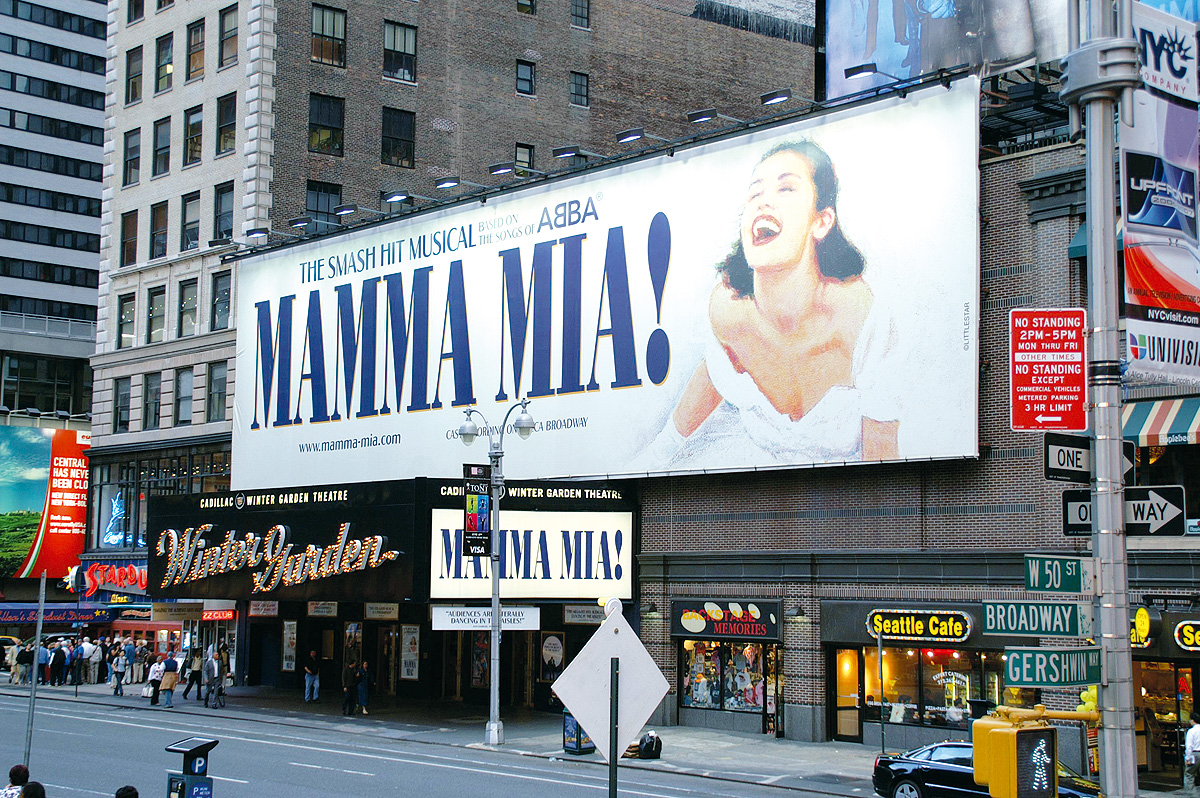
\includegraphics[width=360px]{BroadwayPlayers_01.jpg}
  \caption{A picture of the same gull looking the other way!}
\end{figure}
본 연구에서는 사각형 특징을 이용한 Visual SLAM알고리즘을 제안한다. 기존에 주로 연구되어 온 방법은 점 특징을 이용하는 것으로 영상에서 복수의 특징점을 찾고 매칭하여 카메라의 상대 위치와 자세를 갱신한다. 점 특징 기반의 SLAM은 로봇의 위치 추정과 지도 작성 모두 점을 이용하는 방법이라 할 수 있다. 그러나 점 특징의 특성 상 정보량이 굉장히 적어 SLAM에서 중요하게 다루어지는 data association문제, loop closing 문제에 효과적으로 대처하기 힘들다. 
이 연구에서 제안하는 사각형 특징은 특정한 기하관계를 만족하는 4개의 점이다. 사각형 특징이 평면 위에 존재한다는 가정 하에 특징과 카메라 사이의 homography를 찾는 것으로 다수의 점을 이용하여 essential matrix를 얻는 것을 대체할 수 있다. 이는 지표가 고르지 못한 자연지형이나 

카메라 추적 연구는 시퀀스 상에서 특징점의 대응관계를 기반으로 하기 때문에 검출 및 매칭의 정확도에 의해 시스템 성능이 크게 영향 받는다. 기존 매칭과정에서는 특징 주변의 이미지 패치(patch)간의 상관도(correlation)를 구하거나 카메라 변환 등을 고려한 다해상도 패치의 차분(difference) 연산을 적용한다. 보다 정확한 매칭과 대상 장면의 기술을 위해 SIFT, SURF등의 특징 기술자(descriptor)를 적용하지만, 특징점의 추출과 기술자의 생성에는 많은 연산이 요구되기 때문에 실시간 응용분야에는 적합하지 않다.

사전에 구조화되지 않은 환경에서 평면 등의 기하 정보를 추정하는 기술은 증강현실에서 실제 및 가상 물체간의 상호작용을 위해 중요하다. Chekhlov은 재구성된 3차원 점 클라우드(cloud)로부터 평면 구조를 유추하여 SLAM 맵에 결합하였다[15].
그러나 장면에 대한 맵이 증가하면서 발생하는 누적 오차나 잘못된 매칭 등으로 인한 오차 등은 고려되지 않았다. 시퀀스에서 자동적으로 평면을 검출하기 위한 방법은 일반적으로 호모그래피의 변환 오차를 비교하지만, 이를 판단하기 위한 문턱치(threshold)를 결정하기 어렵다. 또한 특징 집합으로 구성되는 동일 평면들을 구별하는 반복 투표(voting) 방법은 계산이 많기 때문에 실시간 분야에 활용되기 어렵다.
Simon은 게임 등의 실시간 활용을 위해 평면을 검출하고 이를 재구성하는 방법을 제안했다[16].
대상 영상을 격자(grid)로 나누고 허프(hough) 변환의 국소 최대치(local maxima)를 구하여 동일 평면에 해당하는 사각형을 선택한다. 동일 사각형의 클러스터(cluster)와 참조 평면과의 교차선 영역을 구하며, 이를 이용해 3차원 위치와 방향정보를 구한다. 그러나 참조 평면을 구성하는 이미지의 2차원 다각형은 사용자의 수작업을 통해 설정하며, 실제 공간에 적용한 결과
를 제시하지 못했다. 


목표 1 : robust rectangle detection in perspective image
본 연구에서 제안하는 SLAM 방법에 사용할 직사각형 특징을 추출하는 기술을 개발한다. 알려지지 않은 투영구조를 가진 이미지에서 사변형 특징을 검출하고 perspective warp되기 이전에 직사각형으로서의 제약조건을 만족하는 사변형을 찾는다. 연속된 scene에서 일관된 특징이 추출될 수 있도록 검출된 특징을 refine한다. 

목표 2 : Scalable SLAM with rectangle feature
직사각형 특징을 이용한 SLAM알고리즘으로 도심지와 같은 환경에서의 large-scale SLAM문제와 복도나 방 안과 같은 환경에서의 small-scale SLAM문제를 동시에 해결할 수 있는 scalableSLAM 기술을 연구한다. 

목표 3 : real-time SLAM using coupled line camera calibration method that finds homography analytically 
기존의 많은 연구에서는 epipolar geometry를 통해 얻은 essential matrix에 특이값 분해를 통해 camera의 motion estimation을 수행하였다. 본 연구에서는 coupled line camera를 이용한 camera calibration 기법으로 해석적인 방법으로 homography를 얻어 보다 빠르게 motion estimation을 수행

visual SLAM은 자율이동로봇의 주행 뿐 아니라 웨어러블 컴퓨팅, 사용자 인터페이스, 증강 현실, 로봇 수술 등의 분야에 응용된다. 


\chapter{EKF-SLAM Framework를 이용한 사각형 특징 기반의 Visual SLAM}

\section{SLAM Framework}
영상 위의 사변형을 구성하는 각 점을 가우시안 확률변수로 표현
\[
y_t=\begin{bmatrix}
X_t & m
\end{bmatrix}^T
\]
\[
X_t=\begin{bmatrix}
x & y & z & \textbf{q}
\end{bmatrix}^T
\]
\[
m_i=\begin{bmatrix}
x_i & y_i & z_i & \textbf{q}_i
\end{bmatrix}^T
\]
\[
u_t=\begin{bmatrix}
v_x & v_y & v_z &  q_{\omega,u} &  q_{x,u} &  q_{y,u} & q_{z,u}
\end{bmatrix}^T
\]
where $\textbf{q}=\begin{bmatrix}\eta & \epsilon_x & \epsilon_y & \epsilon_z\end{bmatrix}^T $ a quaternion 
\[
Z_t^i = \begin{bmatrix}N(u_i, \sigma_{u_i}) \\ N(v_i, \sigma_{v{_i}})\end{bmatrix}, \quad i=0,1,2,3.
\]
Note. Normal distribution can be represented by following form,
\[
N(\mu,\sigma)=\frac{1}{\sqrt{2\pi\sigma}}\exp{-\frac{(x-\mu)^2}{2\sigma}}
\]
CLC 혹은 동등한 사각형 복원 알고리즘을 이용하여 상대자세를 복원
\[
f(Z_t^i)=\begin{bmatrix} x_t^i & y_t^i & z_t^i & \textbf{q}_t^i & s_t^i \end{bmatrix}^T, \quad
\]


\section{EKFSLAM}
\[
p(f(z_t) | X_t ,m)=\prod^K_{i=1}p(f(z_t^i) | c_t^i, X_t, m)
\]
\[ 
p(X_t | f(Z_t^i), c_t^i, m) = \eta \, p(f(Z_t^i) | c_t^i, X_t, m)p(X_t | c_t^i, m)
\]
\[
p(f(Z_t^i) | c_t^i, X_t, m) = N(x_t^i-\hat{x})\cdot N(y_t^i-\hat{y})\cdot N(z_t^i-\hat{z})\cdot N(\textbf{q}_t^i-\hat{\textbf{q}}) \cdot N(s_t^i-\hat{s})
\]
%where
%\[\hat{r}=\sqrt{(m_{c_t^i,x}-x)^2 + (m_{c_t^i,y}-y)^2 (m_{c_t^i,z}-z)^2},\]
%\[\hat{\phi} = \arccos{\frac{m_{c_t^i,z}-z}{\hat{r}}}, \quad \hat{\varphi}=\arctan{(y/x)}\]

\subsection{Sensor model for rectangle feature}
Prediction:
\[
\hat{x}_{k|k-1}=f(\hat{x}_{k-1|k-1}, u_k)
\]
\[
P_{k|k-1}=\frac{\partial{f}}{\partial{x}}P_{k-1|k-1}\frac{\partial{f}}{\partial{x}}^T + Q_k
\]
Correction:
\[
\tilde{y_k}=z_k-h(\hat{x}_{k|k-1})
\]
\[
S_k=\frac{\partial{h}}{\partial{x}}P_{k|k-1}\frac{\partial{h}}{\partial{x}}^T + R_k
\]
\[
K_k=P_{k|k-1}\frac{\partial{h}}{\partial{x}}^T S_k^{-1}
\]
\[
\hat{x}_{k|k}=\hat{x}_{k|k-1}+K_k\tilde{y}_k
\]
\[
P_{k|k}=(1-K_k\frac{\partial{h}}{\partial{x}})P_{k|k-1}
\]
\[
f(x_{t-1}, u_t)= x_{t-1} \oplus u_t
\]
\[
z_i=h(x_v, m_i)=m_i\ominus(x_v\oplus x_s)
\]
\section{Jacobian $\frac{\partial y}{\partial u} $}
참고 : Quaternion과 rotation matrix사이의 관계
\[R(\textbf{q})=
\begin{bmatrix}
\eta^2+\epsilon_x^2-\epsilon_y^2-\epsilon_z^2 & 2(\epsilon_x \epsilon_y - \eta \epsilon_z) & 2(\epsilon_x \epsilon_z + \eta \epsilon_y) \\
2(\epsilon_x \epsilon_y + \eta \epsilon_z) & \eta^2-\epsilon_x^2+\epsilon_y^2-\epsilon_z^2 & 2(\epsilon_y \epsilon_z - \eta \epsilon_x) \\
2(\epsilon_x \epsilon_z - \eta \epsilon_z) & 2(\epsilon_y \epsilon_z + \eta \epsilon_x)  & \eta^2-\epsilon_x^2-\epsilon_y^2+\epsilon_z^2
\end{bmatrix}
\]
\[
\xi = \begin{bmatrix}
u_x & u_y & u_z & \omega_x & \omega_y & \omega_z
\end{bmatrix}^T =
\begin{bmatrix}
\textbf{u} & \omega
\end{bmatrix}^T
\]
\\

\subsection{Jacobian Matrices of 3D Pose with Quaternion}

\[X_t =  f(X_{t-1}, u_t)= X_{t-1}\oplus u_t
\]
\[=
\begin{bmatrix}
x_{t-1} + (q_{\omega,{t-1}}^2	+ q_{x,t-1}^2- q_{y,t-1}^2- q_{z,t-1}^2) v_x	+ 2( q_{x,t-1}  q_{y,t-1} - q_{\omega,{t-1}} q_{z,t-1})v_y		+ 2( q_{x,t-1}  q_{z,t-1} + q_{\omega,{t-1}} q_{y,t-1})v_z \\
y_{t-1} + 2( q_{x_t-1}  q_{y,t-1}	+ q_{\omega,{t-1}}  q_{z,t-1}) v_x		+ (q_{\omega,{t-1}}^2- q_{x,t-1}^2+ q_{y,t-1}^2- q_{z,t-1}^2)v_y	+ 2( q_{y,t-1}  q_{z,t-1} - q_{\omega,{t-1}}  q_{x,t-1}) v_z \\
z_{t-1} + 2( q_{x,t-1}  q_{z,t-1}	- q_{\omega,{t-1}}  q_{y,t-1}) v_x		+ 2( q_{y,t-1}  q_{z,t-1} + q_{\omega,{t-1}}  q_{x,t-1})v_y		+ (q_{\omega,{t-1}}^2- q_{x,t-1}^2- q_{y,t-1}^2+ q_{z,t-1}^2)v_z \\

q_{\omega_{t-1}}  q_{\omega,u} 	- q_{x_{t-1}}  q_{x,u} - q_{y_{t-1}}   q_{y,u} 		 		- q_{z_{t-1}}  q_{z,u}  \\
q_{x_{t-1}}  q_{\omega,u} 		+ q_{\omega_{t-1}}  q_{x,u} 	- q_{z_{t-1}}  q_{y,u} + q_{y_{t-1}}   q_{z,u} 		 \\
 q_{y_{t-1}}   q_{\omega,u} +q_{z_{t-1}}  q_{x,u} 				+ q_{\omega_{t-1}}  q_{y,u} 	 	- q_{x_{t-1}}  q_{z,u} \\
q_{z_{t-1}}  q_{\omega,u} - q_{y_{t-1}}   q_{x,u} 	+ q_{x_{t-1}}  q_{y,u} + q_{\omega_{t-1}}  q_{z,u}		\\
\end{bmatrix}
\]
\[
{\frac{\partial f}{\partial x}}\bigg| = \begin{bmatrix}
\frac{\partial f_v}{\partial x_v} 	&	\mathbf{0}_{7\times7}	&	\cdots	\\
\mathbf{0}_{7\times7}		&	\mathbf{I}_{7\times7}		&	\cdots	\\
\vdots		&	\vdots	&	\ddots	\\
\end{bmatrix}
\]
\[
{\frac{\partial f_v}{\partial x_v}}\bigg|_{7\times7} = \begin{bmatrix}
\frac{\partial x_v}{\partial x} 		& \frac{\partial x_v}{\partial y} 			& \frac{\partial x_v}{\partial z} 			& \frac{\partial x_v}{\partial q_\omega} 		& \frac{\partial x_v}{\partial q_x} 		& \frac{\partial x_v}{\partial q_y} 		& \frac{\partial x_v}{\partial q_z} \\
\frac{\partial y_v}{\partial x} 		& \frac{\partial y_v}{\partial y} 			& \frac{\partial y_v}{\partial z} 			& \frac{\partial y_v}{\partial q_\omega} 		& \frac{\partial y_v}{\partial q_x} 		& \frac{\partial y_v}{\partial q_y} 		& \frac{\partial y_v}{\partial q_z} \\
\frac{\partial z_v}{\partial x} 		& \frac{\partial z_v}{\partial y} 			& \frac{\partial z_v}{\partial z} 			& \frac{\partial z_v}{\partial q_\omega} 		& \frac{\partial z_v}{\partial q_x} 		& \frac{\partial z_v}{\partial q_y} 		& \frac{\partial z_v}{\partial q_z} \\
\frac{\partial q_{\omega,v}}{\partial x} & \frac{\partial q_{\omega,v}}{\partial y} 	& \frac{\partial q_{\omega,v}}{\partial z} 	& \frac{\partial q_{\omega,v}}{\partial q_\omega} & \frac{\partial q_{\omega,v}}{\partial q_x} & \frac{\partial q_{\omega,v}}{\partial q_y} & \frac{\partial q_{\omega,v}}{\partial q_z} \\
\frac{\partial q_{x,v}}{\partial x} 		& \frac{\partial q_{x,v}}{\partial y} 		& \frac{\partial q_{x,v}}{\partial z} 		& \frac{\partial q_{x,v}}{\partial q_\omega} 		& \frac{\partial q_{x,v}}{\partial q_x} 		& \frac{\partial q_{x,v}}{\partial q_y} 		& \frac{\partial q_{x,v}}{\partial q_z} \\
\frac{\partial q_{y,v}}{\partial x} 		& \frac{\partial q_{y,v}}{\partial y} 		& \frac{\partial q_{y,v}}{\partial z}		 & \frac{\partial q_{y,v}}{\partial q_\omega} 	& \frac{\partial q_{y,v}}{\partial q_x} 		& \frac{\partial q_{y,v}}{\partial q_y} 		& \frac{\partial q_{y,v}}{\partial q_z} \\
\frac{\partial q_{z,v}}{\partial x} 		& \frac{\partial q_{z,v}}{\partial y} 		& \frac{\partial q_{z,v}}{\partial z}		 & \frac{\partial q_{z,v}}{\partial q_\omega}		 & \frac{\partial q_{z,v}}{\partial q_x} 		& \frac{\partial q_{z,v}}{\partial q_y} 		& \frac{\partial q_{z,v}}{\partial q_z} \\
\end{bmatrix}
=
\begin{bmatrix}
\mathbf{I}_{3\times3} & A \\
\mathbf{0}_{4\times3} & B
\end{bmatrix}
\]
\[
A=
2\begin{bmatrix}
  q_{\omega,t-1} v_x  -q_{z,t-1} v_y   +  v_z q_{y,t-1} 	& q_{z,t-1} v_x  + q_{\omega,t-1} v_y  - q_{x,t-1} v_z 	& - q_{y,t-1} v_x  + q_{x,t-1} v_y  +   q_{\omega,t-1} v_z \\
  q_{x,t-1} v_x  + q_{y,t-1} v_y  + q_{z,t-1} v_z 		& q_{y,t-1} v_x  - q_{x,t-1} v_y  -q_{\omega,t-1} v_z 	&  q_{z,t-1} v_x +  q_{\omega,t-1} v_y -   q_{x,t-1} v_z  \\
  -q_{y,t-1} v_x + q_{x,t-1} v_y  + q_{\omega,t-1}  v_z	& q_{x,t-1} v_x  + q_{y,t-1} v_y  +  q_{z,t-1} v_z 		& - q_{\omega,t-1} v_x + q_{z,t-1} v_y -   q_{y,t-1} v_z \\
  -q_{z,t-1} v_x - q_{\omega,t-1} v_y  + q_{x,t-1} v_z 	& q_{\omega,t-1} v_x - q_{z,t-1} v_y  +  q_{y,t-1} v_z 	&  q_{x,t-1} v_x  - q_{y,t-1} v_y -  q_{z,t-1} v_z \\
\end{bmatrix}^T
\]
\[B=
\begin{bmatrix}
 q_{\omega,u}& - q_{x,u}& - q_{y,u}& - q_{z,u}\\
 q_{x,u}&  q_{\omega,u}&  q_{z,u}& - q_{y,u}\\
 q_{y,u}& - q_{z,u}&  q_{\omega,u}&  q_{x,u}\\
 q_{z,u}&  q_{y,u}& - q_{x,u}&  q_{\omega,u}
\end{bmatrix}
\]
\\
\[
{\frac{\partial f_v}{\partial u}}\bigg|_{7\times7} =
\begin{bmatrix}
C & \mathbf{0}_{3\times3} \\
\mathbf{0}_{4\times3} & D
\end{bmatrix}
\]

\[
C=
\begin{bmatrix}
 q_{\omega,t-1}^2 +  q_{x,t-1}^2 -  q_{y,t-1}^2 -  q_{z,t-1}^2		& 2  q_{x,t-1}  q_{y,t-1} - 2  q_{\omega,t-1}  q_{z,t-1}			& 2  q_{\omega,t-1}  q_{y,t-1} + 2  q_{x,t-1}  q_{z,t-1}			\\
2 q_{\omega,t-1}  q_{z,t-1} + 2  q_{x,t-1}  q_{y,t-1}			&  q_{\omega,t-1}^2 -  q_{x,t-1}^2 +  q_{y,t-1}^2 -  q_{z,t-1}^2	& 2  q_{y,t-1}  q_{z,t-1} - 2  q_{\omega,t-1}  q_{x,t-1}			\\
2 q_{x,t-1}  q_{z,t-1} - 2  q_{\omega,t-1}  q_{y,t-1}			& 2  q_{\omega,t-1}  q_{x,t-1} + 2  q_{y,t-1}  q_{z,t-1}			&  q_{\omega,t-1}^2 -  q_{x,t-1}^2 -  q_{y,t-1}^2 +  q_{z,t-1}^2	\\
\end{bmatrix}\]
\[D=
\begin{bmatrix}
q_{x,t-1}& -q_{x,t-1}& -q_{y,t-1}& -q_{z,t-1}\\
q_{x,t-1}&  q_{\omega,t-1}& -q_{z,t-1}& q_{y,t-1}\\
q_{y,t-1}&  q_{z,t-1}&  q_{\omega,t-1}&-q_{x,t-1}\\
q_{z,t-1}& -q_{z,t-1}&  q_{y,t-1}&q_{\omega,t-1}\\
\end{bmatrix}
\]

\subsection{Jacobian $\frac{\partial h}{\partial x} $}
sensor model은 아래와 같다.
\[
z_i=h(x_v, m_i)=m_i\ominus(x_v\oplus x_s)
\]
이 때 
\[
\frac{\partial h}{\partial x} =
\begin{bmatrix}
\frac{\partial h_1}{\partial x_v} & \frac{\partial h_1}{\partial y_1} & 0 & 0&\cdots\\
\frac{\partial h_2}{\partial x_v} & 0 & \frac{\partial h_2}{\partial y_2} & 0&\cdots\\
\frac{\partial h_3}{\partial x_v} & 0 & 0 &  \frac{\partial h_3}{\partial y_3}&\cdots\\
\vdots&\vdots&\vdots&\vdots&\ddots
\end{bmatrix}
\]

\subsection{Exponential Map - Rotation Matrix}
$\xi\in\textrm{se}$(3)일 때
$SE(3)$와 아래와 같은 관계가 성립한다. 
\[
\exp(\xi) = \begin{bmatrix} \textbf{R} & \textbf{V}u \\ \textbf{0} & 1 \end{bmatrix}, 
\textbf{R} = \textbf{I} + A\omega_X + B\omega_X^2, \textbf{V}=\textbf{I} + B\omega_X + B\omega_C^2\]
\[
\theta=\sqrt{\omega^T\omega}, A = \frac{\sin\theta}{\theta}, B=\frac{1-\cos\theta}{\theta^2}, C=\frac{1-A}{\theta^2}
\]
\[
\textbf{R} = 
\begin{bmatrix}
 1+B(\omega_2^2-\omega_3^2)	&  -A\omega_3 -B\omega_1\omega_2	& A\omega_2 - B\omega_1\omega_3 \\
 A\omega_3+B\omega_1\omega_2	& 1-B(\omega_1^2+\omega_3^2)		& A\omega_1 + B\omega_2\omega_3 \\
A \omega_2-B\omega_1\omega_3	& -A\omega_1 - B\omega_2\omega_3	& 1-B(\omega_1^2-\omega_2^2)
 \end{bmatrix}
\]
\[
\textbf{V} = 
\begin{bmatrix}
 1+C(\omega_2^2-\omega_3^2)	&  -A\omega_3 -C\omega_1\omega_2	& A\omega_2 - C\omega_1\omega_3 \\
 A\omega_3+C\omega_1\omega_2	& 1-C(\omega_1^2+\omega_3^2)		& A\omega_1 + C\omega_2\omega_3 \\
A \omega_2-C\omega_1\omega_3	& -A\omega_1 - C\omega_2\omega_3	& 1-C(\omega_1^2-\omega_2^2)
 \end{bmatrix}
\]
practical approach로 $\mathbf{R}^6\rightarrow SE(3)$대신 $\mathbf{R}^6\rightarrow R\times S^3$를 이용하고 컴퓨터의 정밀도 오차를 고려하여 matrix exponential의 급수 전개를 제한하여 계산상의 편의를 얻는 방법이 있다.

\chapter{Data Association}

\chapter{실험결과}

\chapter{결론}
dd

\chapter{부록}
dd

% references section

% can use a bibliography generated by BibTeX as a .bbl file
% BibTeX documentation can be easily obtained at:
% http://www.ctan.org/tex-archive/biblio/bibtex/contrib/doc/
% The IEEEtran BibTeX style support page is at:
% http://www.michaelshell.org/tex/ieeetran/bibtex/
%\bibliographystyle{IEEEtran}
% argument is your BibTeX string definitions and bibliography database(s)
%\bibliography{IEEEabrv,../bib/paper}
%
% <OR> manually copy in the resultant .bbl file
% set second argument of \begin to the number of references
% (used to reserve space for the reference number labels box)

\bibliographystyle{IEEEtran}%...는 bst 파일의 이름(확장자 없이)
\bibliography{ThesisBibTeX.bib}%...는 bib 파일의 이름(확장자 없이)
%\begin{thebibliography}{1}
%\bibitem{greenberg}
%A. Greenberg, J. Hamilton, D.A. Maltz, and P. Patel,
%\emph{The cost of a Cloud: Research Problems in Data Center Networks},
%ACM SIGCOMM Computer Communication Review (CCR), 
%Vol. 39, No. 1, pp. 68-73, January 2009.
%
%\bibitem{wallin}
%S. Wallin, V. Leijon, 
%\emph{Telecom Network and Service Management: An Operator Survey}, 
%MMNS, 2009.
%
%\bibitem{hscalability}
%Wikipedia, \emph{Horizontal Scalability},
%\url{http://en.wikipedia.org/wiki/Scalability#Scale_horizontally_.28scale_out.29}
%
%\end{thebibliography}


\chapter*{감사의 글}

감사의 글을 적으시면 되겠습니다.
감사합니다.

\begin{flushright}
\vspace{1cm}
이재민 배상
\end{flushright}

\end{document}


